%&self-intro_kataoka-nagi_20210315
% ↑ use precompiled file

% @file           self-intro_kataoka-nagi_20210315.tex
% @brief          self-intro in data engineering lab
% @author         Kataoka Nagi
% @date           2021-03-14 16:31:05
% $Version:       1.0
% @par            History
%                 New file
% Copyright (c) 2021 Kataoka Nagi
% - This src is released under the MIT License, see LICENSE.
%
%
% \documentclass[dvipdfmx, 11pt]{beamer}^
% aspectratio = 43, 149, 169
% font size = 8pt, 9pt, 10pt, 11pt, 12pt, 14pt, 17pt, 20pt

% @see 「Beamer columns 環境で画像を配置するベストな方法」https://qiita.com/t_uda/items/8ef173eebf9827305135#3-columns-%E7%92%B0%E5%A2%83%E3%81%AE%E6%AD%A3%E3%81%97%E3%81%84%E4%BD%BF%E3%81%84%E6%96%B9
\PassOptionsToClass{hiresbb}{graphicx}
\documentclass[aspectratio=169, dvipdfmx, 14pt, xcolor={svgnames,dvipsnames}]{beamer}
\usepackage{graphicx}
\newcommand{\thickhrulefill}{\leavevmode\leaders\hrule depth-1.2pt height 3.2pt\hfill\kern0pt}
\newcommand{\indicatewidth}[1]{\thickhrulefill{#1}\thickhrulefill}
\newlength{\mytotalwidth}
\mytotalwidth=\dimexpr\linewidth-5mm
\newlength{\mycolumnwidth}
\mycolumnwidth=\dimexpr\mytotalwidth-5mm

\usepackage{base_kataoka-nagi}
\usepackage{slides_kataoka-nagi}
% \usepackage{../styles/base_kataoka-nagi/base_kataoka-nagi} % debug
% \usepackage{../styles/slides_kataoka-nagi/slides_kataoka-nagi} % debug

% precompile preamble from here. don't precompile with glossaries-env!
% type [eptex -ini -jobname="FILE_NAME" "&platex" mylatexformat.ltx FILE_NAME.tex] in cd
% @see 「beamerのコンパイル速度を上げる」 http://margaret-sdpara.blogspot.com/2019/11/beamer.html
\endofdump

% \includeonlyframes{current} % current build \begin{frame}[label=current]

\title[データ工学研究室 自己紹介]{データ工学研究室}
\subtitle{自己紹介}
\author[片岡 凪]{AL18036 片岡 凪}
% \institute[SIT]{芝浦工業大学 工学部 情報工学科 4年}
\institute[AL18036]{芝浦工業大学 データ工学研究室 B3}
\date{March 15, 2021}

\begin{document}
\maketitle

% \begin{frame}[label=current]{\quad 略歴}
\begin{frame}{\quad 略歴}
  \begin{columns}[totalwidth=\mytotalwidth]
    \begin{column}[t]{0.8\mycolumnwidth}
      \begin{itemize}
        \item 千葉県浦安市在住
        \item デジクリ 元代表(デジタル創作)
        \item 芝鯖 元副代表 (サバゲー)
        \item Twitter @calm\_IRL
        \item Github  KataokaNagi
      \end{itemize}
    \end{column}
    \begin{column}[T]{0.2\mycolumnwidth}
      \centering
      
\includegraphics[width=80pt]{img/icon.jpg}
    \end{column}
  \end{columns}
\end{frame}

\begin{frame}{\quad 不真面目な話}
  \begin{columns}[totalwidth=\mytotalwidth]
    \begin{column}[t]{0.8\mycolumnwidth}
      \begin{itemize}
        \item ゲーム
              \begin{itemize}
                \item Among usやスマブラをゆるくプレイ
              \end{itemize}
        \item アニメ
              \begin{itemize}
                \item 今期は8作品も観るものがあって大変
              \end{itemize}
        \item Vtuber
              \begin{itemize}
                \item リスニング能力を鍛えようとしたら\\先月hololive JPの沼に落ちた (???)
              \end{itemize}
        \item ガジェット
              \begin{itemize}
                \item 給付金は全てオーディオに消えた
              \end{itemize}
      \end{itemize}
    \end{column}
    \begin{column}[T]{0.2\mycolumnwidth}
      \centering
      
\includegraphics[width=100pt]{img/icon_marsh.png}
    \end{column}
  \end{columns}
\end{frame}

\begin{frame}{\quad 真面目な話}
  \begin{columns}[totalwidth=\mytotalwidth]
    \begin{column}[t]{0.8\mycolumnwidth}
      \begin{itemize}
        \item スキル
              \begin{itemize}
                \item Java,C++,Python,LaTeX,数学
              \end{itemize}
        \item 競プロ
              \begin{itemize}
                \item AtCoderをプレイ中
                \item Kaggleもやってみたい
              \end{itemize}
        \item 関心分野
              \begin{itemize}
                \item ゲームやWebサービスの制作
                \item 画像や説明可能なAI?
              \end{itemize}
        \item Discordで話そう
              \begin{itemize}
                \item 心理的安全性の高い研究室ライフをみんなで!
              \end{itemize}
      \end{itemize}
    \end{column}
    \begin{column}[T]{0.2\mycolumnwidth}
      \centering
      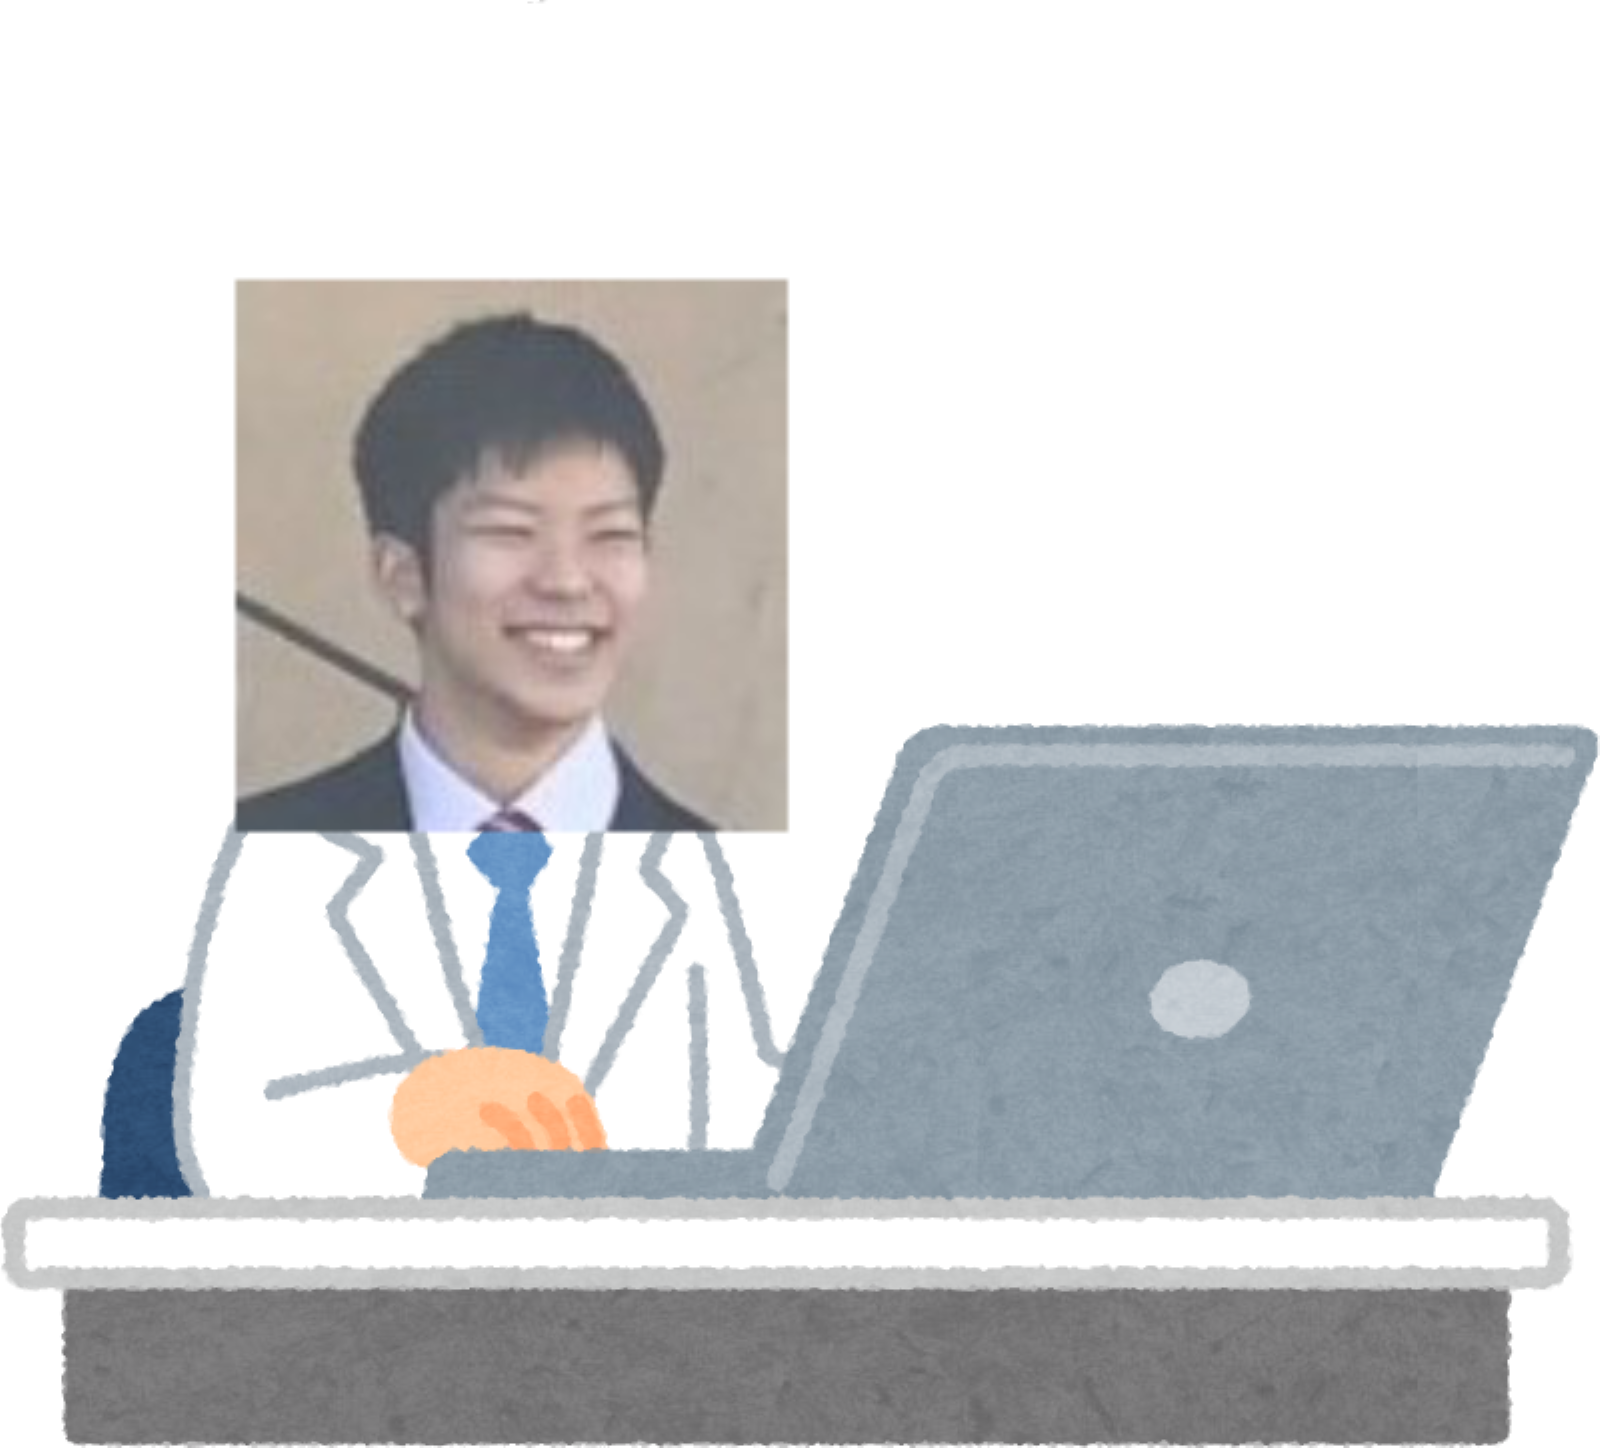
\includegraphics[width=100pt]{img/icon_pc.png}
    \end{column}
  \end{columns}
\end{frame}

\end{document}
